% Superday Topic B -- principles part.  XeLaTeX:  latexmk -xelatex principles.tex
% Layout spec: talk/superday/OUTLINE.md.  Experiment facts: research/coldstart_C01/PLAN.md.
\documentclass[t,20pt]{beamer}
\geometry{paperwidth=13.333in,paperheight=7.5in}

% Metropolis inner / outer / colour themes; fonts are set below (Fira Sans + Fira Math from the TeX tree).
\useinnertheme[sectionpage=none,subsectionpage=none]{metropolis}
\useoutertheme[progressbar=none,numbering=none]{metropolis}
\usecolortheme{metropolis}
\usefonttheme{professionalfonts}

\usepackage{fontspec}
\usepackage{unicode-math}
\setsansfont{FiraSans}[Extension=.otf, UprightFont=*-Book, ItalicFont=*-BookItalic,
  BoldFont=*-SemiBold, BoldItalicFont=*-SemiBoldItalic]
\setmainfont{FiraSans}[Extension=.otf, UprightFont=*-Book, ItalicFont=*-BookItalic,
  BoldFont=*-SemiBold, BoldItalicFont=*-SemiBoldItalic]
\setmonofont{FiraMono}[Extension=.otf, UprightFont=*-Regular, BoldFont=*-Medium]
\newfontfamily\mediumfont{FiraSans}[Extension=.otf, UprightFont=*-Medium, ItalicFont=*-MediumItalic]
\setmathfont{FiraMath-Regular.otf}
\newfontfamily\cjkfont{FandolHei-Regular.otf}   % only for one Chinese file name in a source note

\usepackage{tikz}
\usetikzlibrary{arrows.meta,positioning,calc,fit,decorations.markings}
\usepackage{array,booktabs,colortbl}
\usepackage{fancyvrb}

% ------------------------------------------------------------------ colours (OUTLINE.md)
\definecolor{ink}{HTML}{2E2E2E}
\definecolor{sec}{HTML}{6B6B6B}
\definecolor{rulec}{HTML}{C8C8C8}
\definecolor{accent}{HTML}{1F5A96}
\setbeamercolor{normal text}{fg=ink,bg=white}
\setbeamercolor{background canvas}{bg=white}
\setbeamercolor{frametitle}{fg=ink,bg=white}
\setbeamercolor{alerted text}{fg=accent}
\setbeamercolor{structure}{fg=ink}
\arrayrulecolor{rulec}
\setlength{\heavyrulewidth}{0.9pt}
\setlength{\lightrulewidth}{0.9pt}

% ------------------------------------------------------------------ sizes (points are literal: the page is 13.333 x 7.5 in)
\newcommand\titlesize{\fontsize{32}{38}\selectfont}
\newcommand\secsize{\fontsize{16}{20}\selectfont}
\newcommand\nodesize{\fontsize{16}{19}\selectfont\hyphenpenalty=10000\exhyphenpenalty=10000}
\newcommand\notesize{\fontsize{14}{17}\selectfont\hyphenpenalty=10000\exhyphenpenalty=10000}
\newcommand\pnsize{\fontsize{12}{14}\selectfont}

% ------------------------------------------------------------------ grid
\setbeamersize{text margin left=0.85in,text margin right=0.85in}
\setbeamertemplate{navigation symbols}{}
\setbeamertemplate{headline}{}
% Frame title: a fixed-height box, baseline 0.92 in from the top on every page (strut fixes the baseline).
\setbeamertemplate{frametitle}{%
  \nointerlineskip
  \vbox to 1.30in{%
    \vskip 0.50in
    \hbox{{\mediumfont\titlesize\color{ink}\rule{0pt}{0.42in}\insertframetitle}}%
    \vss}%
}
% Page number: bottom right, 12 pt, mid-gray, right edge on the right text margin.
\setbeamertemplate{footline}{%
  \hbox to \paperwidth{\hfill{\pnsize\color{sec}\insertframenumber}\hskip 0.85in}%
  \vskip 0.36in}
\setlength{\parindent}{0pt}
\setlength{\parskip}{0pt}

% ------------------------------------------------------------------ text helpers
\newcommand\key[1]{{\mediumfont\color{accent}#1}}
\newcommand\lead[1]{{\mediumfont #1}}
\newcommand\illus{{\notesize\itshape\color{sec}illustrative}}
\newcommand\file[1]{{\ttfamily\detokenize{#1}}}
\newcommand\sub[1]{\par\vspace{5pt}{\raggedright\secsize\color{sec}#1\par}}
\newenvironment{blist}{%
  \begin{list}{\textcolor{sec}{\textbullet}}{\def\makelabel##1{##1\hfil}%
    \setlength\leftmargin{0.34in}\setlength\labelwidth{0.2in}\setlength\labelsep{0.14in}%
    \setlength\itemsep{16pt}\setlength\parsep{0pt}\setlength\topsep{0pt}\setlength\partopsep{0pt}%
    \setlength\itemindent{0pt}\setlength\listparindent{0pt}\setlength\rightmargin{0pt}}}%
  {\end{list}}
\newcounter{nl}
\newenvironment{nlist}{%
  \begin{list}{\textcolor{sec}{\arabic{nl}}}{\usecounter{nl}\def\makelabel##1{##1\hfil}%
    \setlength\leftmargin{0.40in}\setlength\labelwidth{0.26in}\setlength\labelsep{0.14in}%
    \setlength\itemsep{26pt}\setlength\parsep{0pt}\setlength\topsep{0pt}\setlength\partopsep{0pt}%
    \setlength\itemindent{0pt}\setlength\listparindent{0pt}\setlength\rightmargin{0pt}}}%
  {\end{list}}
\newcolumntype{L}[1]{>{\raggedright\arraybackslash}p{#1}}
\newcommand\thead[1]{\leavevmode{\mediumfont\color{sec}#1}}
\newcommand\gap[1]{\par\vspace{#1}}
% content top: tables and figures start on the frame's top line; a first text line or a [t] minipage is lifted onto it
\newcommand\textfirst{\vspace*{-0.14in}}
\newcommand\colsfirst{\vspace*{-0.37in}}
\newcommand\colsafter{\par\vspace{-0.24in}}
% figures sit on the text block: left edge on the left margin, width exactly the text width
\newcommand\fig[1]{\par\noindent\makebox[\textwidth][l]{\input{#1}}\par}
\AtBeginDocument{\hyphenpenalty=10000\exhyphenpenalty=10000\raggedright}

% ------------------------------------------------------------------ figures: one line width, Stealth tips, square corners
\tikzset{
  x=1in, y=1in,
  >={Stealth[length=7pt,width=5.5pt]},
  every picture/.style={line width=0.9pt},
  grid/.style={trim left=0in, trim right=11.633in-0.9pt},
  box/.style={rectangle, draw=ink, line width=0.9pt, minimum height=0.68in, align=center,
              font=\nodesize, text=ink, inner sep=4pt},
  cb/.style={box},                                  % code part
  lb/.style={box, draw=accent},                     % LLM / Partura part
  pb/.style={box, draw=sec, dashed, text=sec},      % planned, not built
  tint/.style={fill=accent!10},                     % the single 10 % accent tint per figure
  arr/.style={->, line width=0.9pt, draw=ink},
  arrl/.style={->, line width=0.9pt, draw=accent},
  lab/.style={font=\nodesize, text=sec, inner sep=2pt},
  labl/.style={font=\nodesize, text=accent, inner sep=2pt},
  ann/.style={font=\notesize, text=sec, inner sep=1.5pt},        % 14 pt figure annotations
  annl/.style={font=\notesize, text=accent, inner sep=1.5pt},
  anni/.style={font=\notesize, text=ink, inner sep=1.5pt},
  guide/.style={draw=rulec, dotted, line width=0.9pt},            % dotted alignment guides
  mask/.style={fill=white},                                       % label background over a line
  t10/.style={fill=accent!10}, t20/.style={fill=accent!20}, t28/.style={fill=accent!28}, t35/.style={fill=accent!35},
}

\begin{document}

% ================================================================== 1 Title
\begin{frame}[plain]
\begin{tikzpicture}[remember picture,overlay]
  \node[anchor=base west, inner sep=0, align=left, text=ink]
    at ($(current page.north west)+(0.85in,-2.45in)$)
    {\mediumfont\titlesize Partura: an LLM research loop\\[2pt]\mediumfont\titlesize that steers a symbolic alpha miner};
  \node[anchor=base west, inner sep=0, text=sec]
    at ($(current page.north west)+(0.85in,-3.45in)$)
    {Principles: task, agents, loop, steering interface, evaluation protocol, tokens};
  \draw[rulec] ($(current page.north west)+(0.85in,-3.85in)$) -- ++(11.633in,0);
  \node[anchor=base west, inner sep=0, text=ink]
    at ($(current page.north west)+(0.85in,-4.45in)$) {Xiangyu Wang};
  \node[anchor=base west, inner sep=0, text=sec, font=\secsize]
    at ($(current page.north west)+(0.85in,-4.90in)$) {Trexquant Superday \,·\, Topic B \,·\, October 2026};
  \node[anchor=base east, inner sep=0, text=sec, font=\pnsize]
    at ($(current page.south east)+(-0.85in,0.36in)$) {1};
\end{tikzpicture}
\end{frame}

% ================================================================== 2 Outline
\begin{frame}{Outline}
\textfirst
\begin{nlist}
  \item \lead{Principles} \,—\, this part
    \sub{Why tokens should buy beliefs, not candidates; task; searcher; agents; one round; steering;\\how the system is measured; tokens; integrity; status; known limitations}
  \item \lead{Results} \,—\, \key{in progress: C01 is running}
    \sub{C01 cold-start comparison: AlphaCube alone (A) vs.\ AlphaCube + Partura (B); one bad-signal case}
  \item \lead{Limitations and next steps}
    \sub{What the results do and do not show; what changes before the next experiment}
\end{nlist}
\end{frame}

% ================================================================== 3 Two speeds
\begin{frame}{Search is cheap, belief is expensive}
\textfirst
LLMs should not write thousands of formulas. They should form beliefs\\
and change \key{where a cheap searcher looks}.
\gap{0.30in}
\fig{figs/loop.tex}
\end{frame}

% ================================================================== 4 Tokens buy beliefs
\begin{frame}{Tokens should buy beliefs, not candidates}
\fig{figs/cost.tex}
\gap{0.30in}
Spend tokens only where an LLM adds value: \key{reading results, revising beliefs,}\\
\key{and compiling them into search interventions}.
\end{frame}

% ================================================================== 5 Task specification
\begin{frame}{Task specification}
\fig{figs/task.tex}
\gap{0.16in}
\lead{Signal}\quad $s_{i,t} = x(\mathcal{D}_{\le t})_i$ \quad {\secsize\color{sec}one number per stock $i$ and day $t$, known after the close of day $t$}
\gap{0.10in}
\lead{Return}\quad $r_{i,t+1} = P_{i,t+2}/P_{i,t+1} - 1$ \quad {\secsize\color{sec}$P$: first-15-minute VWAP; missing if limit-up at the open}
\gap{0.10in}
{\secsize\color{sec}Given: Claude agents (Opus 5.5, Opus 5, Sonnet 5, Haiku 5.5) under a finite token budget; AlphaCube GP;\\
long-only top decile, 15 bp per side; \textcolor{accent}{the search sees 2018-01-02 to 2023-08-07 only}.}
\end{frame}

% ================================================================== 6 Signal card
\begin{frame}{A finished output is a signal card}
\begingroup\secsize
\renewcommand\arraystretch{1.45}%
\begin{tabular}{@{}L{2.0in}L{6.0in}L{3.3in}@{}}
\toprule
\thead{Field} & \thead{Content} & \thead{Filled by} \\
\midrule
\lead{Thesis} & mechanism, counterparty, falsifiable prediction, condition under which it fails & \textcolor{accent}{Lead (Opus 5)}, signed off by the Coordinator \\
\lead{Implementation} & expression $x$; sign and half-life fixed on train; signal after the close of $t$, trade at the open of $t+1$ & searcher (GP) + reward code \\
\lead{Evidence} & train / valid score; one test read (net excess, $t$); style-neutral read; turnover; $|\rho|$ to the known family & deterministic code \\
\lead{Provenance} & guidance file, round, seed, code hashes, ledger entry & code (\file{evidence.json}, ledger) \\
\midrule
\multicolumn{3}{@{}l@{}}{\illus\quad the known family as a card: thesis “volatile intraday turnover marks illiquid, speculative names”;} \\[-4pt]
\multicolumn{3}{@{}l@{}}{\phantom{\illus}\quad $x$ = \file{cross_mean(day_std(Amt), 30)}, sign $-1$; evidence and provenance written by code} \\
\bottomrule
\end{tabular}
\endgroup
\gap{0.36in}
Done = all four fields filled \key{and the one test read logged in the ledger}.
\end{frame}

% ================================================================== 7 Searcher as a black box
\begin{frame}{The searcher is a black box with three handles}
\textfirst
Partura never edits AlphaCube. It reaches the search only through \key{three ports}.
\gap{0.22in}
\fig{figs/searcher.tex}
\gap{0.22in}
Fixed and identical in both arms: reward \file{long}, budget $N = 192$, population 48,\\
depth 2–4, random seed, operator library (286 searchable operators).
\end{frame}

% ================================================================== 8 Agent roles
\begin{frame}{Agent roles}
\begingroup\secsize
\renewcommand\arraystretch{1.16}%
\begin{tabular}{@{}L{1.50in}L{1.00in}L{2.60in}L{3.60in}L{2.25in}@{}}
\toprule
\thead{Role} & \thead{Model} & \thead{Reads} & \thead{Writes} & \thead{May not} \\
\midrule
\textcolor{accent}{\lead{Coordinator}} & Opus 5.5 & arm B digest; Lead’s YAML, cards & plan: 1–3 questions and tasks; final: edit or veto, \file{beliefs_r<k>.md}, seeds & change reward, pool, budget, rules \\
\textcolor{accent}{\lead{Executors}} & Sonnet 5 & digest; arm B evidence; kernels & findings for the Lead (1–3, parallel) & write to the repo \\
\textcolor{accent}{\lead{Lead}} & Opus 5 & digest; questions; findings & \file{C01_r<k>.yaml}, \file{cards_r<k>.md}; runs the check & read arm A, old findings \\
\textcolor{accent}{\lead{Checker}} & Haiku 5.5 & check-script output & exit 0 = admissible & edit files \\
\lead{Scripts, GPU} & code & evidence; transcripts & digest (arm B only), 16 jobs, token ledger & open the test segment \\
\lead{Judge} & code & heads; test segment once & verdict by fixed rules & change after run 1 \\
\bottomrule
\end{tabular}
\endgroup
\gap{0.28in}
Proposer ≠ judge: \key{the agents that write a thesis never score it}; scoring is code\\
with rules fixed before the first run.
\end{frame}

% ================================================================== 9 One round
\begin{frame}{One round of the loop}
\fig{figs/seq.tex}
\end{frame}

% ================================================================== 10 Belief to intervention
\begin{frame}[fragile]{From belief to intervention}
\fig{figs/bars.tex}
\colsafter
\vspace{0.10in}
\begin{minipage}[t]{5.6in}
\raggedright
\vspace{0pt}
$q(x) \;\propto\; p(x)\, w(x), \qquad w(x) = \prod_{r \in R(x)} w_r$
\gap{0.12in}
$\Pr[\text{accept } x] = \min\!\bigl(1,\; w(x)/w_{\mathrm{ref}}\bigr)$
\gap{0.12in}
$w_{\mathrm{ref}} = \max\bigl(1, \max_r w_r\bigr), \qquad \text{ban:}\ w_r = 0$
\end{minipage}%
\hspace{0.35in}%
\begin{minipage}[t]{5.68in}
\raggedright
\vspace{0pt}
{\notesize\color{sec}one rule in full, as Partura writes it \enspace\itshape illustrative}
\gap{4pt}
\begin{Verbatim}[formatcom=\color{ink}, fontsize=\fontsize{14}{17}\selectfont]
- id: P1
  action: weight
  w: 2.0
  pattern: "day_skew(_)"
  why: "<one falsifiable sentence>"
  evidence: ["<a C01 run of arm B>"]
\end{Verbatim}
\end{minipage}
\end{frame}

% ================================================================== 11 Matched-budget A/B
\begin{frame}{Measuring the system, not a signal}
\fig{figs/matrix.tex}
\gap{0.22in}
Per arm: 3 rounds × $K = 8$ seeds × $N = 192$ = \key{4,608 paid evaluations}.
\end{frame}

% ================================================================== 12 Decision rules
\begin{frame}{Decision rules, fixed before any run}
\fig{figs/dedup.tex}
\colsafter
\begin{minipage}[t]{6.55in}
\raggedright
\vspace{0pt}
\lead{Discovery}\enspace score$(x) = \min(\mathrm{SR}_{\mathrm{train}}, \mathrm{SR}_{\mathrm{valid}}) \ge 1.0$
\gap{0.10in}
\lead{Head}\enspace $|\rho(x,k)| < 0.5$ and $\max_h |\rho(x,h)| < 0.7$
\sub{$h$: the heads kept so far;\\
$k$: the known family \file{cross_mean(day_std(Amt), 30)}}
\gap{0.10in}
\lead{Valid}\enspace net excess $> 0$ and $t = \mathrm{SR}\cdot\sqrt{T} \ge 2.0$
\sub{test segment, read once; SR: long-only net-excess Sharpe; $T$: years}
\end{minipage}%
\hspace{0.30in}%
\begin{minipage}[t]{4.78in}
\raggedright
\vspace{0pt}
\begingroup\secsize
\renewcommand\arraystretch{1.30}%
\begin{tabular}{@{}L{1.75in}L{2.85in}@{}}
\toprule
\thead{Verdict} & \thead{Condition} \\
\midrule
\textcolor{accent}{\lead{Partura helps}} & $n_B - n_A \ge 2$ and\newline $n_B \ge 2\max(n_A, 1)$ \\
\lead{Partura is worse} & $n_A - n_B \ge 2$ \\
\lead{Cannot tell} & otherwise \\
\bottomrule
\end{tabular}
\gap{8pt}
\color{sec}$n_A, n_B$: valid heads per arm, all rounds;\\secondary metrics never change the verdict.
\endgroup
\end{minipage}
\end{frame}

% ================================================================== 13 Tokens
\begin{frame}{Token accounting}
\vspace*{-0.10in}
$T_k = \sum_{a \in \mathcal{C}_k} \bigl(\tau^{\mathrm{in}}_a + \tau^{\mathrm{cw}}_a + \tau^{\mathrm{cr}}_a + \tau^{\mathrm{out}}_a\bigr), \qquad T_A = 0, \qquad T_B = T_2 + T_3$
\sub{$\mathcal{C}_k$: agent calls before round $k$; $\tau$: input, cache-write, cache-read, output tokens. Also: $T_B/n_B$, $T_B$ per GPU-hour.}
\gap{0.18in}
\fig{figs/tiers.tex}
\gap{0.20in}
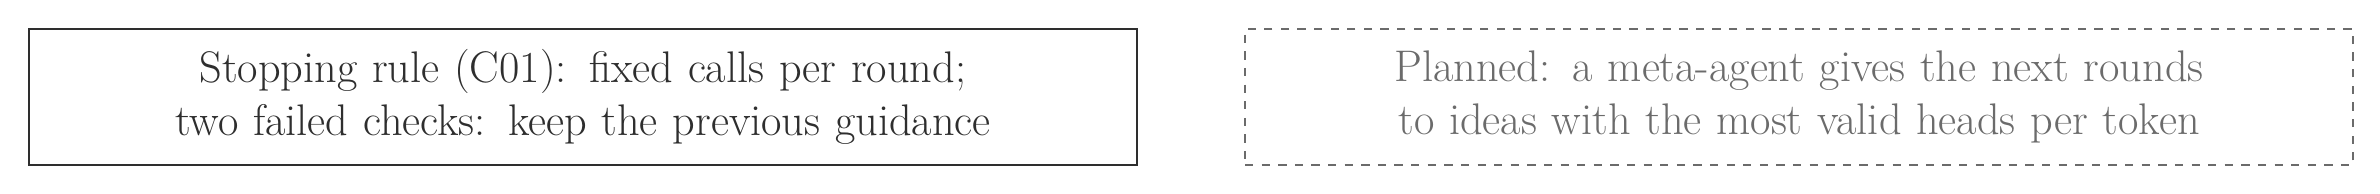
\begin{tikzpicture}[grid]
  \node[cb, minimum width=5.54in, text width=5.39in, anchor=west] at (0,0)
    {{\mediumfont Stopping rule (C01):} fixed calls per round;\\two failed checks: keep the previous guidance};
  \node[pb, minimum width=5.54in, text width=5.39in, anchor=east] at (11.633,0)
    {{\mediumfont Planned:} a meta-agent gives the next rounds\\to ideas with the most valid heads per token};
\end{tikzpicture}
\end{frame}

% ================================================================== 14 Integrity
\begin{frame}{Integrity: what keeps the loop honest}
\begingroup\secsize
\renewcommand\arraystretch{1.36}%
\begin{tabular}{@{}L{2.9in}L{8.55in}@{}}
\toprule
\thead{Mechanism} & \thead{How it is enforced} \\
\midrule
\lead{Rules before runs} & PLAN written before any run; later changes only as a dated revision section \\
\lead{Cold start} & agents read only C01’s own evidence, the PLAN and the code; transcripts audited \\
\lead{Information barrier} & the digest holds arm B only: a deployed system has no control arm \\
\lead{Direction fixed on train} & sign and half-life chosen on train, reused unchanged on valid and test \\
\lead{Ledgered holdout} & test segment read once per head, after R3; each read appended to a ledger \\
\lead{Costs} & 15 bp per side; long-only top decile measured against the equal-weight market \\
\lead{Immutable raw results} & evidence never overwritten; a crash is rerun once, unchanged, and logged \\
\bottomrule
\end{tabular}
\endgroup
\gap{0.40in}
\key{No run is repeated because its result looks bad.}
\end{frame}

% ================================================================== 15 Status
\begin{frame}{Implemented vs.\ planned}
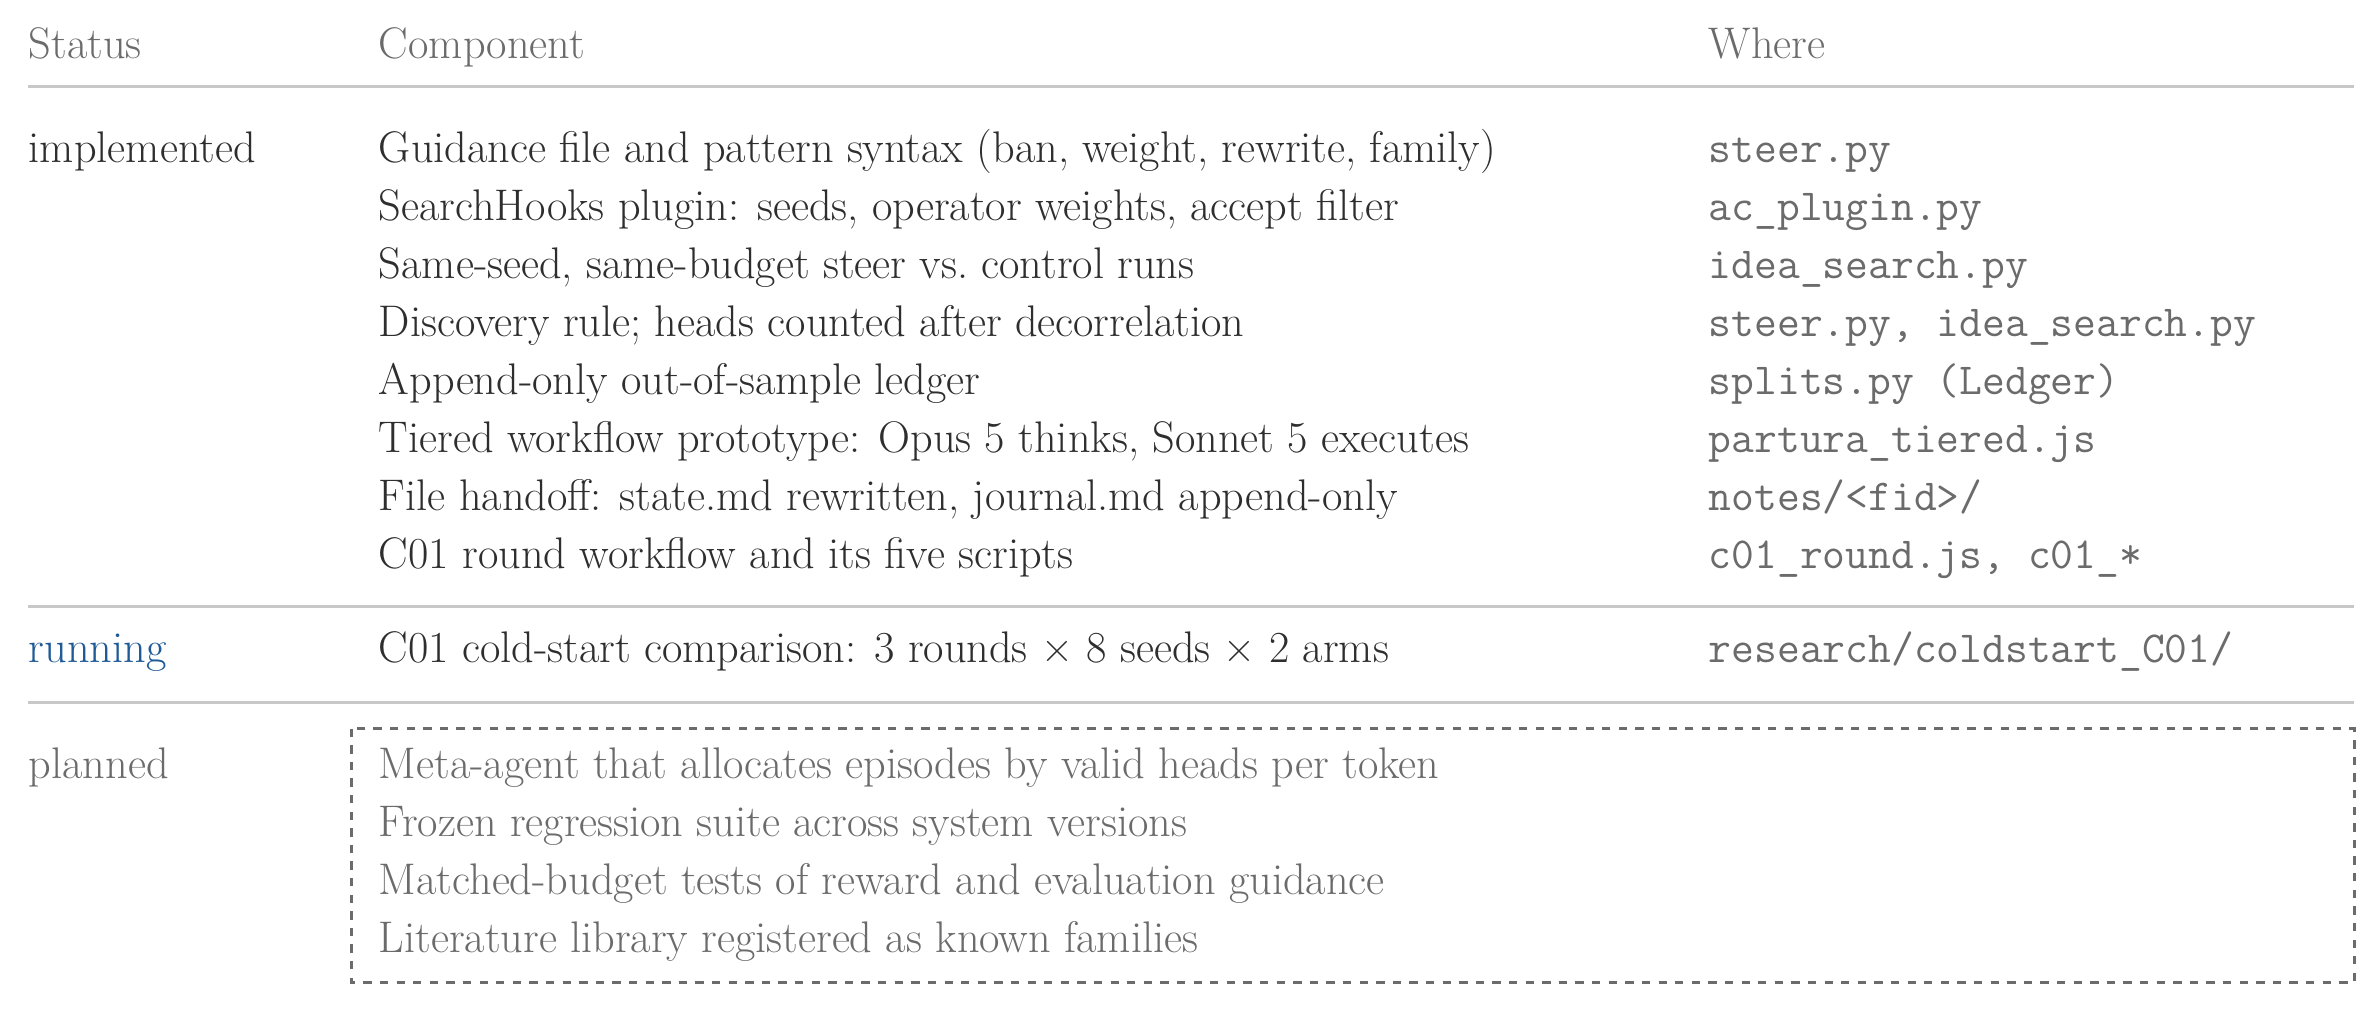
\begin{tikzpicture}[grid]
  \def\P{0.29}
  \tikzset{t/.style={anchor=base west, font=\nodesize, inner sep=0}}
  \node[t, text=sec] at (0,0.22) {\mediumfont Status};
  \node[t, text=sec] at (1.75,0.22) {\mediumfont Component};
  \node[t, text=sec] at (8.40,0.22) {\mediumfont Where};
  \draw[rulec] (0,0.08) -- (11.633,0.08);
  \foreach \k/\c/\w in {
      0/{Guidance file and pattern syntax (ban, weight, rewrite, family)}/{steer.py},
      1/{SearchHooks plugin: seeds, operator weights, accept filter}/{ac\_plugin.py},
      2/{Same-seed, same-budget steer vs.\ control runs}/{idea\_search.py},
      3/{Discovery rule; heads counted after decorrelation}/{steer.py, idea\_search.py},
      4/{Append-only out-of-sample ledger}/{splits.py (Ledger)},
      5/{Tiered workflow prototype: Opus 5 thinks, Sonnet 5 executes}/{partura\_tiered.js},
      6/{File handoff: state.md rewritten, journal.md append-only}/{notes/<fid>/},
      7/{C01 round workflow and its five scripts}/{c01\_round.js, c01\_*}} {
    \node[t, text=ink] at (1.75,-0.30-\k*\P) {\c};
    \node[t, text=sec, font=\nodesize\ttfamily] at (8.40,-0.30-\k*\P) {\w};
  }
  \node[t, text=ink] at (0,-0.30) {\mediumfont implemented};
  \draw[rulec] (0,-2.52) -- (11.633,-2.52);
  \node[t, text=accent] at (0,-2.80) {\mediumfont running};
  \node[t, text=ink] at (1.75,-2.80) {C01 cold-start comparison: 3 rounds × 8 seeds × 2 arms};
  \node[t, text=sec, font=\nodesize\ttfamily] at (8.40,-2.80) {research/coldstart\_C01/};
  \draw[rulec] (0,-3.00) -- (11.633,-3.00);
  \node[t, text=sec] at (0,-3.38) {\mediumfont planned};
  \foreach \k/\c in {
      0/{Meta-agent that allocates episodes by valid heads per token},
      1/{Frozen regression suite across system versions},
      2/{Matched-budget tests of reward and evaluation guidance},
      3/{Literature library registered as known families}} {
    \node[t, text=sec] at (1.75,-3.38-\k*\P) {\c};
  }
  \draw[sec, dashed] (1.62,-3.13) rectangle (11.633,-4.40);
\end{tikzpicture}
\gap{0.18in}
Dashed = design, not built. \key{Only the first group is called implemented.}
\end{frame}

% ================================================================== 16 Limitations
\begin{frame}{Known limitations, stated before the results}
\textfirst
\begin{blist}
  \item \lead{Survivorship.} Every name in the store survives to its last day; no delisted stocks.
    \sub{Biases absolute long-only returns of small, illiquid names upward. \textcolor{accent}{Both arms share it,\\so the A/B comparison holds.}}
  \item \lead{A-shares, long-only.} T+1, limit-up names cannot be bought, shorting is impractical.
    \sub{Label, costs and universe all change in another market.}
  \item \lead{Test segment seen by the designer} in earlier research, not by this experiment.
    \sub{The forward segment is clean but only about 0.7 years long.}
  \item \lead{Power.} 8 seeds may still not separate the arms.
    \sub{One GP configuration gave test Sharpe +0.76 and −0.91 under two seeds. “Cannot tell” is reported as such.}
  \item \lead{Scope.} Only priors and ideas are tested; reward and evaluation guidance are not.
\end{blist}
\end{frame}


% ================================================================== 17 The bar for the autonomous loop
\begin{frame}{Where the full pipeline stands today}
\textfirst
The long-only edge survives the clean forward period;\\
the long-short Sharpe roughly halves. This is the bar for the autonomous loop.
\sub{\textcolor{accent}{Outside this experiment: not a C01 result, not produced by Partura.} AlphaCube plus human iterations.}
\gap{0.08in}
\begingroup\secsize
\renewcommand\arraystretch{1.0}%
\setlength\aboverulesep{1pt}\setlength\belowrulesep{2pt}%
\begin{tabular}{@{}L{8.50in}L{2.95in}@{}}
\toprule
\multicolumn{2}{@{}l@{}}{\textcolor{sec}{\lead{Development test period}, 2023-08-08 – 2025-12-31 (581 trading days)}} \\
\textcolor{sec}{Long-only, 1M RMB simulated account, actual A-share fees, vs.\ equal-weight market:\newline excess Sharpe 2.28, excess return +17.0\%/yr, excess max drawdown −7.2\%}
 & \textcolor{sec}{Long-short decile\newline book (15 bp): Sharpe 4.92\textsuperscript{*}} \\
\midrule
\multicolumn{2}{@{}l@{}}{\lead{Clean forward period}, 2026-01-05 – 2026-09-16 (\textasciitilde 0.68 y)} \\
Long-only top-10\% equal-weight net excess\newline (15 bp linear, not the account simulation): {\mediumfont\color{accent}+16.6\%/yr, Sharpe 1.49}
 & Long-short decile\newline book (15 bp): {\mediumfont\color{accent}Sharpe 2.44} \\
\bottomrule
\end{tabular}
\par\vspace{2pt}
{\notesize\color{sec}\textsuperscript{*}\,4.92: smoothed decile long-short after the §18 re-selection, limit-locked cells excluded. In the §11.1 decomposition of the same champion (hl3, unsmoothed), the long-short Sharpe is 3.99 under the original label and 3.65 when longs exclude limit-up-locked and shorts exclude limit-down-locked names. The short leg is not tradable in A-shares.\par}
\vspace{4pt}
{\color{sec}Development numbers: the factor library was mined on 2018–2025, so the test period was seen during mining; configurations were chosen on the training period only. Forward numbers: selection and weights use data up to 2023-08-07 only.\par}
\endgroup
\gap{0.04in}
{\notesize\color{sec}Sources: AlphaCube \texttt{docs/{\cjkfont 可交易回测}.md} §10 \& §18 (lines 225–241, 257, 929); Partura \texttt{research/two\_level/RESULT.md} item 4.}
\end{frame}

\end{document}
